%\qchapter{\textit{Every obstacle is an opportunity.} \vskip 0.1em -
%  Lance Armstrong}{Introduction} 


\qchapter{\textit{If you don't know where you're going, you might not
  get there.} \vskip 0.1em -
  Yogi Berra}{Introduction} \label{chap:intro}

%Progress always involves risks.  You can't steal second base and keep
%  your foot on first.  ~Frederick B. Wilcox 


%\chapter{Introduction}

\cs{T}he past fifteen years have seen a migration from the
government-operated NSFNet to an agglomeration of commercial networks
that communicate with one another to constitute what we commonly refer
to as ``the Internet''.  This data network requires the cooperation of
tens of thousands of independently operated networks that are
nonetheless competing with one another for each other's customers.  In
the midst of this changeable, federated landscape, we as users expect to
be able to reliably communicate with other users of the network at any
time.

Reliable communication between nodes in a network fundamentally depends
on {\em routing}, the process by which some participant discovers paths
to other network destinations.  In the same way that a human might use
routing to plan a course (\eg, using the ``driving directions'' feature
of an online mapping service to discover a path from Boston to New
York), computers on the Internet rely on routing to discover paths
between each other.  There are many reasons why traffic on the Internet
may not reach its intended destination: parts of the network
infrastructure, network systems, and end hosts can all fail, for
example.  Even if all infrastructure and services operate correctly,
though, two endpoints cannot communicate if they cannot discover a path
between them. 

Today's Internet routing infrastructure is unacceptably fragile.  
Among its shortcomings, it converges slowly~\cite{labovitz:ton01} (and
sometimes not at all~\cite{Griffin2002c}); it is often
misconfigured~\cite{Mahajan2002}; it is hard to control and
predict~\cite{Feamster2003e}; and it has weak security
properties~\cite{id-routing-threats}.  This fragility causes
communication on the Internet to be unreliable and unpredictable. A
major contributing factor to this fragility is Internet routing's
configurability.  Internet routing configuration enables competing
networks both to implement policies reflecting complex business
arrangements and to tune routing protocols to maintain good performance
under highly dynamic conditions.  The behavior of Internet routing is
determined almost entirely by the set of configurations distributed
across the routers in the network.  In this sense, it is rather accurate
to think of Internet routing as a massive distributed computation, and
the routing configuration as a complex, distributed program written in a
variety of low-level languages running on a heterogeneous set of
platforms.  This dissertation develops techniques towards making
Internet routing more correct and predictable; much of the dissertation
focuses on how to make configuration less of a harbinger of incorrect
and unpredictable behavior.

Given that there are so many ways for Internet routing to go wrong,
guaranteeing correct and predictable behavior is a daunting task.  Each
new problem seems to merit a point solution that adds complexity to the
routing protocol, making the infrastructure more complex, unpredictable,
and unwieldy.  Worse yet, network operators, protocol designers, and
researchers have adopted a {\em reactive} approach to reasoning about
Internet routing.  The state-of-the-art for configuring Internet routing
typically involves logging configuration changes and rolling back to a
previous version when a problem arises.  The lack of a formal reasoning
framework means that configuring routers is time-consuming, ad hoc, and
error-prone, and it is becoming more so as with the unceasing addition of
new point fixes and ``features''.
%Furthermore, today's routing configuration is based on the manipulation
%of low-level mechanisms (\eg, access control lists, import and export
%filters, etc.), which makes routing configuration tedious, error-prone,
%and difficult to reason about.

This trend is unsettling, especially as the Internet matures and
increasingly becomes a mission-critical part of our communication
infrastructure.  Rather than proposing point solutions to the myriad
problems in Internet routing, this dissertation takes the opposite
approach: we work top-down, first defining a high-level correctness
specification for Internet routing and subsequently developing
techniques to ensure that the routing protocol satisfies this
specification.  Using the correctness specification as a guide, this
dissertation develops techniques that improve the correctness and
predictability of the Internet routing system. We focus on
this problem in the context of non-malicious network operations.  We
develop techniques that help operators and protocol designers reason
about the behavior of today's Internet 
routing system.  Further, we propose architectural and protocol changes
that make the routing protocol itself less likely to behave incorrectly.  This
dissertation proposes two such tools based on {\em proactive} analysis
of static routing configurations.  One of these tools, called \rcc
(``router configuration checker''), uses the correctness specification
and its constraints to derive a set of constraints that it checks
directly against the routing configuration.  The second tool, which we
call a {\em routing sandbox}, allows a network operator to determine how
traffic will flow through the network and quickly evaluate the effects
of configuration changes on the flow of traffic.



%This dissertation develops a systematic framework for reasoning about the
%correct behavior of routing.  While the designers of security protocols
%have long had BAN logic~\cite{Burrows90} to aid in reasoning about the
%properties of a cryptographic protocol, the designers and operators of
%routing protocols have no similar systematic framework that allows them
%to reason about when a routing protocol is likely to behave correctly.

%% \begin{table}[t]
%% \centering
%% {\footnotesize
%% \begin{tabular}{r|p{2in}|p{3.25in}}
%% & {\em Network Management Tools} & {\em Protocol Design and Network
%%   Architecture} \\ 
%%   \hline
%% {\em Static} & \parbox{2in}{{\em rcc} (Ch.~\ref{chap:rcc}) \\
%%   BGP Routing Model (Ch.~\ref{chap:sandbox})} & 
%% \parbox{3.25in}{Stable policy routing (Ch.~\ref{chap:policy}) \\
%%   Preventing MED-induced oscillation
%%   (Ch.~\ref{sec:sandbox:med_disc})} \\ \hline
%% {\em Dynamic} & Detecting contract violations
%%   (Ch.~\ref{sec:dynamic}) & Routing Control Platform
%%   (Ch.~\ref{sec:rcp}) 
%% \end{tabular}
%% }
%% \caption[Major contributions of this dissertation]{Major contributions
%% of this dissertation.  While most of the work in 
%%   this dissertation involves enforcing constraints on the {\em static}
%%   configuration of Internet routing, we also make some contributions
%%   that involve the analysis or design of protocol dynamics.}
%% \label{tab:contributions}
%% \end{table}


While the techniques we present have proved effective for improving the
correctness and predictability of today's Internet routing system, we
firmly believe that the design of the routing infrastructure should
address correctness and predictability as first-order concerns.  The
tools and techniques presented in this dissertation would likely have
been far easier had the routing infrastructure been designed with these
goals in mind in the first place. Consequently, this dissertation also
proposes several architectural and protocol changes towards improving
the robustness and manageability of the system.  In general, we believe
that the correctness specification in this dissertation provides a sound
framework for considering such design changes.
%We
%discuss these contributions in more detail in
%Section~\ref{sec:contributions}.

We begin with a high-level overview of Internet routing to provide some
context.  In Section~\ref{sec:intro:config}, we discuss how routing
configuration can be used to control the behavior of the routing
protocol; we also describe how mistakes and unintended interactions in
routing configuration can induce catastrophic routing failures.  After
discussing the challenges in guaranteeing correct and predictable
Internet routing (Section~\ref{sec:challenges}), we explain how {\em
proactive} techniques for analyzing routing configuration can guarantee
correctness and improve predictability of Internet routing
(Section~\ref{sec:proactive}), summarize the major contributions of this
dissertation (Section~\ref{sec:contributions}) and offer some take-away
lessons (Section~\ref{sec:lessons}) that offer insights that we hope
will prove useful when thinking about further improvements to Internet
routing.
Section~\ref{sec:guide} concludes the chapter with a guide for reading
the rest of this dissertation.


\section{Internet Routing Overview}\label{sec:intro:overview}

\begin{figure}[b!]
\centering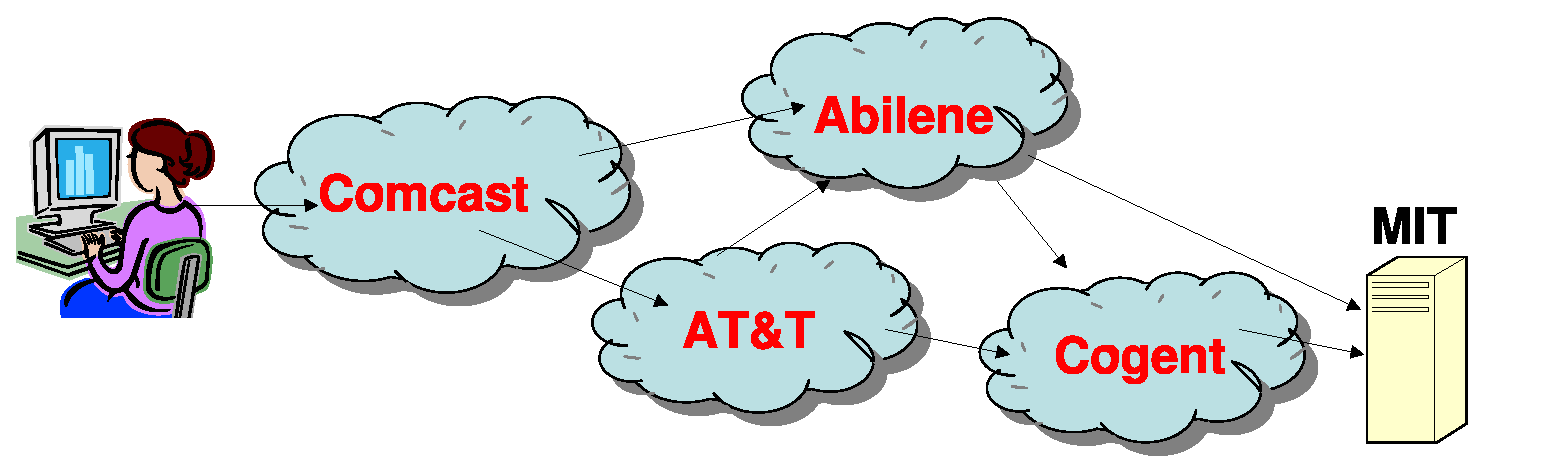
\epsfig{file=figures/overview.eps, width=\linewidth}
\caption[Overview of the Internet's structure]{A typical Internet path may traverse multiple ``Autonomous Systems''.}
\label{fig:intro:overview}
\end{figure}

\begin{figure}[t]
\centering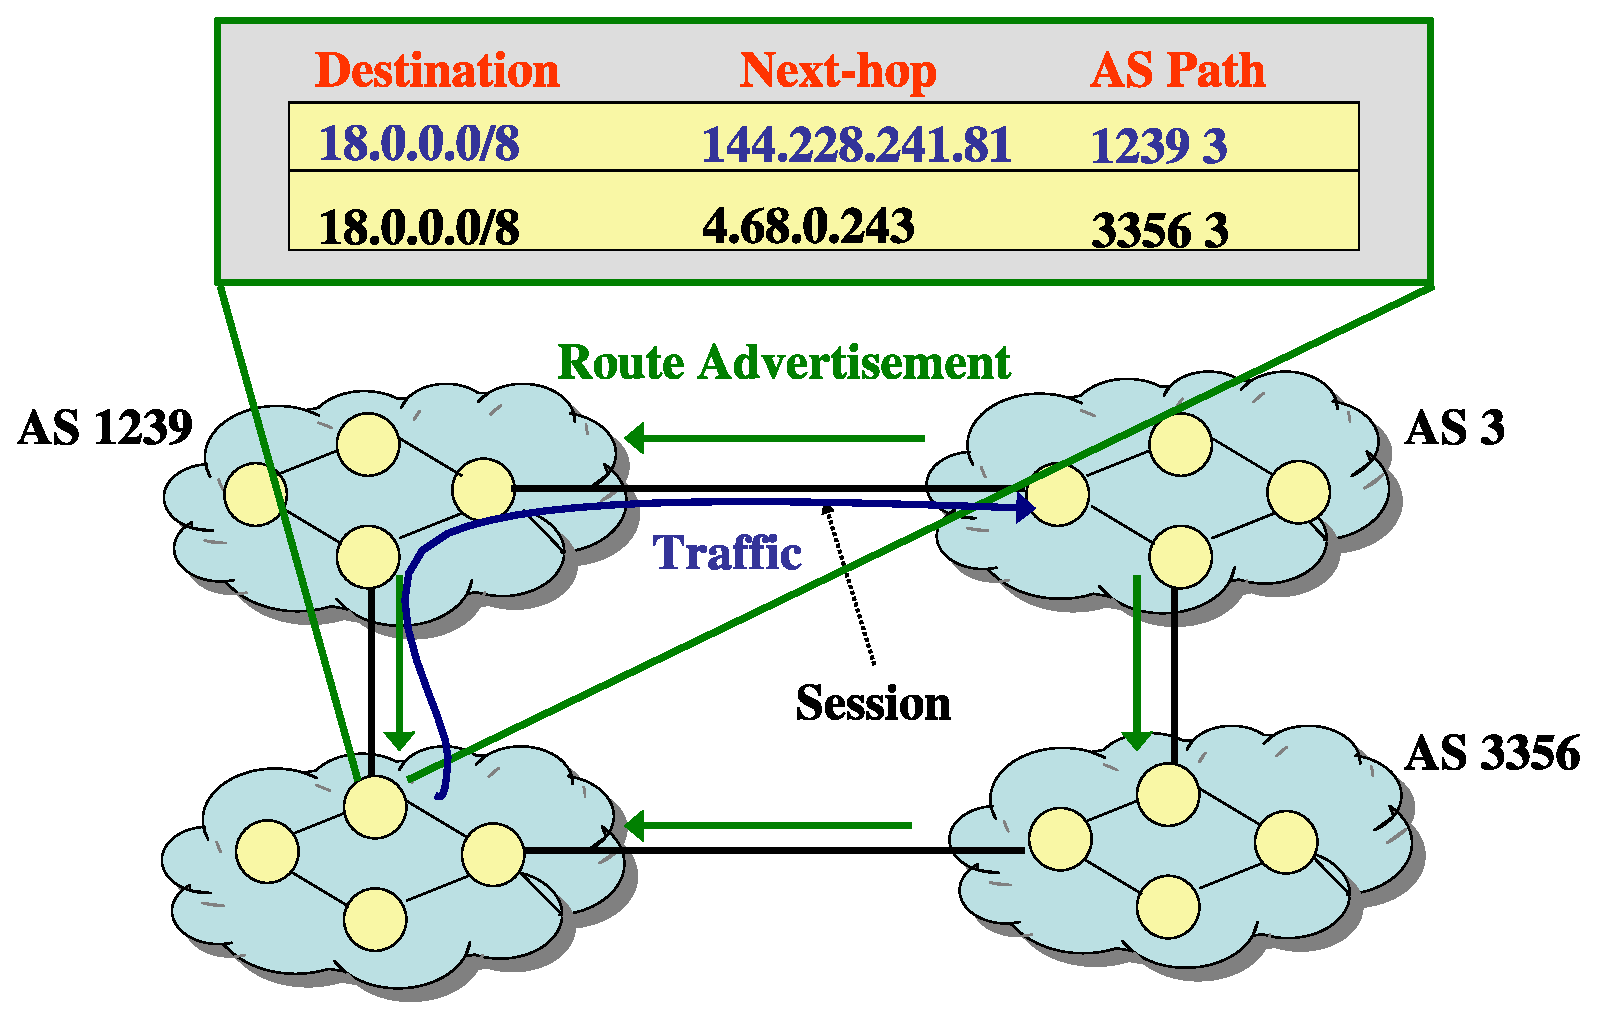
\epsfig{file=figures/rtgtable.eps, width=0.8\linewidth}
\caption[How ASes exchange routing information]{ASes exchange routing
information over BGP {\em sessions} between 
  routers.  A router may learn multiple routes to the destination but
  ultimately selects a {\em single} best route.  Traffic flows in the opposite
  direction of route advertisements.}
\label{fig:intro:rtgtable}
\end{figure}



Although it is common to think of ``the Internet'' as a single, monolithic
network, it is actually composed of tens of thousands of independently
operated networks, commonly called {\em Autonomous Systems} (ASes).
Figure~\ref{fig:intro:overview} shows an example of how traffic from a cable
modem user may traverse multiple ASes en route to machines at MIT.
Internet traffic is forwarded from source to destination through a
sequence of {\em routers} in one or more ASes.  

Each one of these ASes typically has independent (and often
conflicting) economic and performance goals, yet these ASes must cooperate by
exchanging routing information to achieve global connectivity (\eg, to
allow a home user who buys service from his cable modem provider to
communicate with hosts that purchase connectivity from other ASes).
The current routing protocol on the Internet is the Border Gateway
Protocol (BGP)~\cite{rfc1771}.  As shown in
Figure~\ref{fig:intro:rtgtable}, ASes achieve global reachability by
establishing BGP sessions between neighboring ``border'' routers.  Each
AS has may have anywhere from a single router to hundreds of routers. 
%
Each of these routers maintains a {\em routing table}, which contains
one or more routes for each destination.  Each router
selects a single best route to each destination.  Routing on the Internet
is {\em destination-based}; that is, a router selects the next hop (\ie,
router) for which to forward traffic solely based on the destination IP
address of each packet.  The destination for a route is represented in
terms of an IP {\em prefix}, which specifies a group of IP addresses
that share a common number of bits.


\begin{figure*}[tb!]
\begin{center}
\begin{small}
\begin{minipage}{5in}
\begin{verbatim}
   Network          Next Hop            Path
*> 18.0.0.0/8       144.228.241.81      1239 3 
*  18.0.0.0/8       12.0.1.63           7018 3356 3 
\end{verbatim}
\end{minipage}
\end{small}
\end{center}
\caption[Example BGP routing table entry]{BGP routing table entry for
prefix 18.0.0.0/8 as 
  it might appear on a router.  Each BGP route has attributes in
  addition to the next hop IP address and AS path, which we will discuss
  later.}
\label{fig:bgpex}
\end{figure*}


Figure~\ref{fig:bgpex} shows example routing table entries for the set
of destinations represented by the IP prefix {\tt 18.0.0.0/8}, which
represents the $2^{24}$ IP addresses that share the first 24 bits, {\tt
18.*}.  Although each router may learn multiple candidate routes
to a prefix, (\ie, the routing table shown in Figure~\ref{fig:bgpex} has
two possible routes for the same destination), each router ultimately
selects a {\em single} best route for each prefix (in the routing table,
the route that the router ultimately selects is indicated by the ``{\tt
>}''.  The {\em next hop} attribute is the IP address that the router
must forward traffic towards to send traffic along this route.  The
router may learn how to reach this next hop IP address in one of several
ways: a ``static'' route may be hardcoded, the router might learn a
route via a routing protocol that is run inside the AS (\eg, OSPF),
and so forth.  The {\em path} attribute refers to the AS path: the
sequence of ASes that the route advertisement traversed en route to this
router.  
%``Metric'' and ``LocPrf'' refer to the Multiple Exit
%Discriminator (MED) and Local Preference attributes, respectively; an
%operator can manipulate these two attributes to control which route a
%router ultimately selects, given multiple options.  
A BGP route has several additional route attributes that are not
pictured; we will describe
these additional attributes in more detail in Section~\ref{sec:propagation}.

Internet routing requires neighboring ASes to exchange routing
information, but it also requires each of these ASes to run an internal
routing protocol (``Interior Gateway Protocol'', or {\em IGP}) to
establish reachability information about destinations within the same
AS.  For example, in the routing table excerpt shown in
Figure~\ref{fig:bgpex}, the router knows that to forward traffic to any
destination in {\tt 18.*}, it must send the traffic towards the next hop
{\tt 144.228.241.81}.  For ``border'' routers, this next hop is typically
the address of an interface of the router in a neighboring autonomous
system and is an immediate next hop.  Routers within an AS, however,
must use the IGP to discover the outgoing
interface over which to send traffic towards this next hop, which may be
multiple hops away.  This dissertation focuses on BGP but does
not address the operation of internal routing protocols.  Other
work provides more detailed treatment of IGPs~\cite{Feldmann2001,
Shaikh2002, Shaikh2004}.


\section{Configuration: The Achilles' Heel of Internet Routing}
\label{sec:intro:config}

Analyzing the behavior of any routing protocol is inherently difficult,
but Internet routing presents a unique set of challenges because it must
be highly configurable to support the complex economic and performance
goals that each independently operated network is attempting to satisfy.
The standards document for BGP~\cite{rfc1771} specifies the message
format but intentionally leaves unspecified many details, including the
criteria for 
selecting the route to a destination given multiple alternatives.
Instead, these details are left to its {\em configuration}.  In this
section, we 
explain how configuration affects routing protocol behavior; we then
present some examples that demonstrate how configuration mistakes can
induce catastrophic routing failures.

\subsection{How Configuration Affects Routing Protocol Behavior}
\label{ssec:intro:config}

Internet routing configuration provides a network operator remarkable
latitude in controlling how the protocol behaves.  In particular,
Internet routing configuration allows an operator to control the routing
protocol in the following ways:

\begin{itemize}
\item {\bf Which ASes to carry traffic for.}  Depending on the
  business relationships that an AS has established with other
  ASes, it may arrange to carry traffic to a destination for some of
  those ASes but not others~\cite{Gao2001a}.  Routing configuration
  controls which routes an AS advertises to each of its neighbors,
  implicitly controlling which neighbors can send traffic over the
  AS en route to a destination.

\item {\bf How traffic enters and leaves the AS.} An AS
  typically has multiple links over which it can send traffic to a
  destination: some of these links are internal (\ie,
  they are between two routers in the same AS) and others are
  external (\ie, they are between routers in neighboring ASes).
  Changes in traffic demands may cause any of these links to become
  congested.  In response, a network operator may change the routing
  configuration to shift portions of the traffic load to a different set
  of links~\cite{Feamster2002b}. 

\item {\bf How routers within an AS learn routes to external
  destinations.}  Each independently operated network comprises tens to
  hundreds of routers.  Ultimately, every router in the AS must
  learn the routes to external destinations, but, initially, only the
  AS's ``border'' routers learn these routes.  Routing
  configuration controls how the routes propagate from an AS's
  border routers to the rest of the routers in the AS.
\end{itemize}


Changing traffic demands and business relationships, planned
maintenance, and equipment failures may all change traffic patterns
through the AS, but routing protocols do not automatically adapt to
these changing conditions.
As a
result, network operators must constantly tune the behavior of the
routing protocols in their ASes to control how traffic flows through
them.  

\subsection{Problem: Configuration Mistakes Cause Routing Failures}
\label{sec:intro:problem}

The cost of Internet routing's
configurability is a high degree of complexity.  The unfortunate
consequence of this complexity is that the potential for incorrect
behavior is enormous.

The consequences of incorrect behavior can be staggering.  The past few
years alone have seen several high-profile examples of Internet routing
configuration problems:

\begin{itemize}
\item In
1997, a small ISP in Florida configured its routing in a way that caused
all of the Internet's traffic to be routed through it~\cite{www-as7007}.
\item In 2001, Microsoft brought down its Web servers with a routing
misconfiguration; it took nearly a day to diagnose the
problem~\cite{www-microsoft-outage}.  
\item In 2002, Worldcom took down more
than 20\% of its nationwide ``backbone'' in the United States with a
routing configuration problem~\cite{www-worldcom-outage}.  
\item In 2004, Level3 incurred a widespread outage due to a router
configuration problem~\cite{www-l3-outage}.
\item In 2005, an ISP in Bolivia caused a major outage when it announced
the IP prefix for AT\&T's United States backbone
network (\ie, {\tt 12.0.0.0/8}).~\cite{nanog-att}. 
\end{itemize}
Major news outlets report only the most catastrophic routing failures;
in fact, mistakes in routing configuration are continually causing
reasonably serious routing failures.  In the introduction to
Chapter~\ref{chap:rcc}, we 
present the results of our informal study of the mailing list archives
of the North American Network Operators Group (NANOG)~\cite{nanog-list}.
In this study, we 
find that upwards of two-thirds of the routing failures reported on this
mailing list can be attributed to problems with routing configuration.
Network operators are continually misconfiguring routing protocols in
ways that cause such problems as loops, ``blackholes'' (where a router
simply drops traffic en route to some destination because it does not
have a route for it), routing instability, and so forth.  

%%%%%%%%%%%%%%%%%%%%%%%%%%%%%%%%%%%%%%%%%%%%%%%%%%%%%%%%%%%%

\section{Challenges}\label{sec:challenges}

While guaranteeing correct and predictable behavior poses challenges for
any routing protocol, Internet routing presents several unique
challenges.  First, Internet routing has more configurable facets
than traditional routing protocols, many
of which can be misconfigured or otherwise cause the routing protocol to
behave unpredictably.  In order to analyze the correctness of the
routing protocol, we must first define a specification for correct
behavior.  Second, the sheer size of the distributed
router configuration, as well as the fact that the configurations have
dependencies across routers, can give rise to erroneous or unpredictable
behavior.  Third, because each network operator configures his AS
independently of others, the policies defined in one AS may conflict
with those in neighboring ASes.

\subsection{Defining a Correctness Specification}

As described in Section~\ref{ssec:intro:config}, Internet routing
configuration affords a network operator much flexibility in defining
how the protocol operates.  The Cisco configuration language has more
than 1,000 different commands, and a network of 500 routers may have
upwards of one million lines of configuration distributed across the
AS~\cite{www-cisco-ios-master}.  Given the many ways in which an
operator can affect protocol behavior, determining the correctness of
the configuration is a daunting task without a high-level specification
for ``correct'' behavior.  Developing such a specification involves
distilling the high-level properties that the protocol should satisfy
from the protocol's mechanistic detail.

Defining a correctness specification for Internet routing is complicated
by the fact that the protocol's correctness is in part 
based on whether it achieves a network operator's economic
and performance goals.  Unfortunately, these high-level policies are
encoded in terms of mechanistic configuration commands distributed
across hundreds of routers---that is, the specification of the {\em
intended} behavior doesn't even exist in the first place, which makes it
difficult to determine whether the routing configuration indeed induces
the intended behavior.

One motivation for developing a correctness specification for Internet
routing is that the protocol not only ``does the right thing'' when it
satisfies the specification, but a routing protocol that satisfies the
specification is also more predictable.  For example, network operators
often would like to predict the effects of a configuration change on the
behavior of the routing protocol without testing that change on a live
network or running a complex simulator.  Predicting how the protocol
will behave first requires making assumptions about its behavior to
simplify route prediction, but precisely determining the constraints that
are required to simplify route prediction for such a complex protocol is
challenging.

\subsection{Analyzing Complex Configuration}

%% Configuring a network's routing boils down to independently configuring
%% the routers within a network.  Each network contains as many as several
%% hundred routers; each of these routers may have tens of thousands of
%% lines of configuration.  Although an operator configures each of these
%% routers separately, the configuration typically has dependencies across
%% multiple routers in the network.  Furthermore, a network may contain
%% routers from different vendors, each of which have a different
%% configuration language.  The configuration of these routers collectively
%% dictates the behavior of the network. In this sense, configuring a
%% network of routers is not unlike writing a large distributed program in
%% several different flavors of assembly language.  Given this complexity,
%% it is not surprising that network operators make mistakes in configuring
%% routers.

In designing tools that can help network operators reason
about the correctness of Internet routing, we must also design ways
to manage routing configuration's staggering complexity.  First, we must
represent this 
distributed router configuration in a format that is easy to analyze.
Second, we must tackle the engineering problem of parsing the various
routing configuration languages from different vendors and translating
the configurations into this format.

Determining how a configuration change will affect routing is difficult
in practice.  Not only do ASes contain a large number of routers, but
the route that each router ultimately selects for each destination
depends on many factors, including the routes that the AS's ``border''
routers learn from neighboring ASes, the routing topology within the AS
(\ie, both the internal topology, and the internal BGP topology that
controls how routes are disseminated within the AS).  As we discuss in
more detail in Chapter~\ref{chap:sandbox}, various complicating
protocol artifacts prevent informally reasoning about the route that each
router selects.  Thus, network operators need tools and
systematic techniques to assist them in predicting how a particular
routing configuration will affect the flow of traffic through the AS.


\subsection{Providing Global Guarantees with Only Local Information}

While end-to-end connectivity between Internet hosts fundamentally
depends on the {\em global} behavior of the routing system, no single party
has a global view of the Internet routing system. A network operator may
configure the protocol in a way that interacts in unexpected ways with
the configurations in other ASes.  For example, the interactions of
routing policies in neighboring ASes can cause the routing protocol to
oscillate.

One goal of our work is to explore how we can achieve assurances about
the global behavior of the Internet routing system, while still
preserving the {\em autonomy} of each AS.  That is, each network operator
should retain the ability to independently configure his own AS,
but should also be able to gain some assurances about the global behavior of
the routing system, assuming every AS abides by a similar set of
rules.  


%%%%%%%%%%%%%%%%%%%%%%%%%%%%%%%%%%%%%%%%%%%%%%%%%%%%%%%%%%%%


\section{The Role of Proactive, Static Configuration
Analysis}\label{sec:proactive}  

\begin{figure}[t]
\centering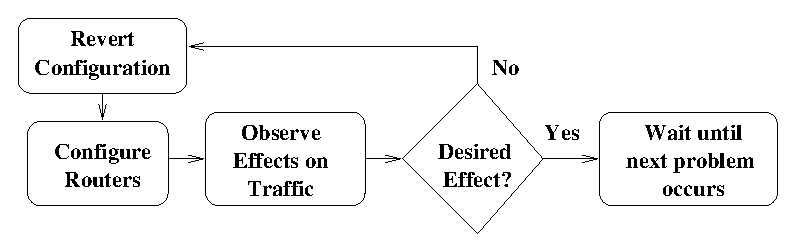
\epsfig{file=figures/workflow.eps, width=0.7\linewidth}
\caption[The state-of-the-art in network configuration management]{The state-of-the-art in network configuration management: {\em
reactive}, ``stimulus-response'' mode of operation.}
\label{fig:intro:workflow}
\end{figure}

Prior to our work, the state-of-the-art in managing Internet routing
protocols was {\em reactive}: the primary way for network operators to
determine the effects of a particular routing configuration (\ie, what
effects that configuration will have on the flow of traffic, or whether
the configuration is even correct in the first place) was to deploy that
configuration on a live network, observe the resulting behavior, and
revert the configuration to a previous version in the event that the
configuration did not produce the desired effects (see
Figure~\ref{fig:intro:workflow}).  This mode of operation has two
shortcomings: First, testing configuration on a live network can cause
unnecessary downtime or poor network performance (and, hence, angry
customers!).  Second, the undesirable effects that result from a
particular configuration may not be immediately apparent when the
configuration is deployed; a failure may only be triggered by the
presence or absence of certain routes.

This dissertation posits that {\em proactive} techniques for analyzing
routing configuration can both prevent a large class of routing failures
and help operators predict and analyze routing protocol behavior.
Changing the workflow from Figure~\ref{fig:intro:workflow} to include a
step that proactively detects problems with routing configuration is
critical for improving the correctness and predictability of Internet
routing.  A remarkable result of our work is that proactive analysis
techniques (\ie, those that analyze the static routing configuration
offline, before it is deployed on a live network) are useful in
detecting configuration faults and efficiently and accurately predicting
the routing protocol's behavior.  In particular, proactive analysis
techniques provide the following benefits over the status quo:

\begin{enumerate}
\itemsep=-1pt
\item {\bf Offline.}  A reactive mode of configuration is time consuming
and can lead to unnecessary performance degradation.  The complexity of
Internet routing makes it essentially impossible to compute
back-of-the-envelope estimates of the effects of configuration changes.
Proactive techniques for determining the correctness and the effects of
Internet routing configuration can help network operators evaluate the
effects of a routing configuration before it is deployed on a live
network.

\item {\bf Accurate.}  Network simulators (\eg,
ns~\cite{www-ns-bgp}, SSFNet~\cite{www-ssfnet}) help operators
understand dynamic routing protocol behavior, but simulation models
network behavior in terms of its protocol dynamics over some certain
period of time.  The {\em outcome} of the simulator will ultimately be
the same as that predicted by static techniques, and the dynamics (which
are nondeterministic) may not necessarily correspond to those in the
actual network anyhow.  Existing simulators do not capture all of the
relevant protocol interactions that may affect correctness, nor do they
explain {\em why} a particular configuration is incorrect.  Because
incorrect behavior sometimes depends on a particular sequence of route
advertisements or may be nondeterministic, correct behavior in a
simulator cannot guarantee correct behavior on a live network.  In this
dissertation, we show that techniques based on direct analysis of static
configuration files can test for necessary or sufficient correctness
conditions and predict the outcome of the routing protocol without
having to simulate the protocol dynamics.

%% While simulators can
%% prove useful, they are often unnecessarily complex: simulators can help
%% an operator study the {\em dynamics} of the network, but operators
%% typically do not care about such dynamics; rather they need to quickly
%% evaluate the {\em outcome} of the route selection process.


\item {\bf Efficient.}  Because network operators cannot use ``back of the
envelope'' calculations to determine what a particular routing
configuration will do, they must often experiment with many
possibilities before arriving at an acceptable solution.  As we will
show in Chapters~\ref{chap:rcc} and~\ref{chap:sandbox}, static analysis
techniques can assist network operators in efficiently determining the
correctness and effects of incremental changes to a routing
configuration.


\end{enumerate}

%% This dissertation presents techniques for determining both the
%% correctness and the outcome of this computation (1)~efficiently, (2)~in
%% a way that facilitates evaluating incremental changes, and (3)~without
%% having to observe the protocol's behavior on a live network.

Analyzing the static router configurations of a single AS proves
surprisingly effective at improving the correctness and predictability
of Internet routing.  An important open question that is {\em not}
addressed in this dissertation involves
exploring the classes of faults that {\em cannot} be detected with
static analysis alone and how analysis of routing {\em dynamics} might
complement static configuration analysis for fault detection and diagnosis.

%% this dissertation also recognizes
%% the limitations of static analysis.  We explore how dynamic analysis of
%% routing protocol messages can complement static configuration analysis,
%% and even changes to the routing protocol and architecture itself.



%%%%%%%%%%%%%%%%%%%%%%%%%%%%%%%%%%%%%%%%%%%%%%%%%%%%%%%%%%%%

\section{Contributions}\label{sec:contributions} 

We now briefly overview the major contributions of this dissertation
before describing each in more detail.  A central contribution of this
dissertation is a formal correctness specification for Internet routing.
We use this specification to derive tests for configuration faults and
as the groundwork for efficient offline analysis of Internet routing.
Using this specification as a guide, we present the design and
implementation of two systems that use proactive configuration analysis
techniques to improve the correctness and predictability of Internet
routing.  The first, \rcc (``router configuration checker''), detects
faults in routing configuration. \rcc helps network operators eradicate
configuration faults before they cause catastrophic routing failures on
a running network. The second, the {\em routing sandbox}, efficiently computes
the routes that each router within a single AS ultimately select, using
only a static snapshot of the routing configuration and network state.
%The
%BGP sandbox allows an operator to experiment with configuration changes
%offline and determine whether a possible configuration change would have
%the desired effect, before deploying the change on a live network.

Because Internet routing inherently involves interaction between
multiple independently operated, competing ASes, some aspects of the
correctness 
specification are difficult to verify by only looking at the
configuration of a single AS in isolation.  In particular, it turns out
to be difficult to determine whether the routing protocol will converge
to a stable route assignment (a property defined as {\em safety} in
previous work~\cite{Varadhan1996}).  Traditional routing protocols
typically satisfy safety, but BGP's {\em policy-based} nature means that
the policies of neighboring ASes can interact to create oscillations.
This dissertation provides the first necessary conditions for
guaranteeing the stability of a policy-based routing protocol.  The rest
of this section discusses these contributions in more detail.

%% While analyzing the static router configurations of a single AS
%% proves surprisingly effective at improving the correctness and
%% predictability of Internet routing, this dissertation also recognizes
%% the limitations of static analysis.  We explore how dynamic analysis of
%% routing protocol messages can complement static configuration analysis,
%% and even changes to the routing protocol and architecture itself.
%% Specifically, we present the design of the Routing Control Platform
%% (RCP), a routing system that separates the route selection logic from
%% the routers themselves and can explicitly guarantee many aspects of the
%% correctness specification.


%This dissertation also makes practical contributions in the areas
%of network management and Internet routing design.  While the
%contributions to network management may prove more immediately
%applicable, we believe that the work more relevant to routing design
%will ultimately make Internet routing intrinsically more robust and
%predictable.  In other words, while network management tools are crucial
%to network operation, our ultimate goal should be to {\em design the
%protocol for manageability}.  Our contributions to routing protocol
%design are a step in the right direction towards this goal.

\subsection{A Correctness Specification for Internet Routing}

We define three high-level properties that a routing
protocol should satisfy. Essentially, all three aspects of this
correctness specification
reflect the following underlying principle: {\em a routing protocol
should propagate 
information that accurately reflects the properties of the underlying
network topology}.  The three properties are as follows:

\begin{itemize}
\item {\bf Route validity.}  If an endpoint learns a route to a
  destination, then that route should correspond to some path.  An
  example of a route validity violation would be a persistent forwarding
  loop: a router learns a route to some destination (\ie, a destination,
  and the next-hop IP address to which traffic should be sent for that
  route), but when it actually attempts to send traffic along that
  route, it is caught in a forwarding loop and never reaches
  the destination.

\item {\bf Path visibility.}  If there exists a sequence of IP-level
  hops (\ie, a {\em path}) from an endpoint to a destination, then
  that endpoint should learn at least one route to that destination.  An
  example of a path visibility violation would be a case where all
  routers inside a fully-connected AS did not learn a route to the
  destination when at least one of those routers learned the route.  

\item {\bf Safety.}  This property requires that the
  routing protocol ultimately assigns a route to each node in the
  Internet graph 
  such that no node has a more preferred available route to the
  destination that it would rather use.  Safety is important not only
  because a routing protocol that persistently oscillates can cause lost
  and reordered packets, but also because it is incredibly difficult to
  diagnose problems when the routing protocol is changing independently
  of the underlying topology.  A violation of safety would be an
  oscillation caused by conflicting policies from different ASes (rather
  than due to topological changes), as described in previous
  work~\cite{Griffin2002c, Varadhan1996}.
\end{itemize}

Chapter~\ref{chap:rlogic} formalizes each of these
properties, as well as well as other concepts (\eg, path,
route, etc.).  Path visibility and route validity are violated primarily
because of configuration complexity, and safety is violated because the
configurations of one AS may interact in unexpected ways with
configurations of other ASes.

Although this dissertation applies this correctness specification to
Internet routing, these properties should prove valuable for analyzing
any routing protocol.  Applying these properties to routing in other
areas (\eg, wireless or sensor networks) is beyond the scope of our
work, but is ripe for exploration.

\subsection{Systems for Proactive Fault Detection and Route Prediction}

This dissertation recognizes a critical missing piece in the {\em
workflow} of configuring today's networks: the step at which network
operators evaluate the effects of a routing configuration before
deploying and running it on a live network.


\begin{figure}[t]
\centering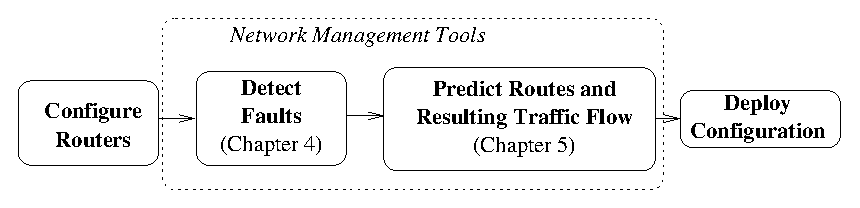
\epsfig{file=figures/workflow2.eps, width=0.75\linewidth}
\caption[This dissertation's contributions in fault detection and
route prediction.]{This dissertation develops two tools for fault detection
  and route prediction.  These tools should be used to analyze the
  behavior of routing configuration before it is deployed on a live
  network.}
\label{fig:intro:workflow2}
\end{figure}


\begin{figure}[t]
\centering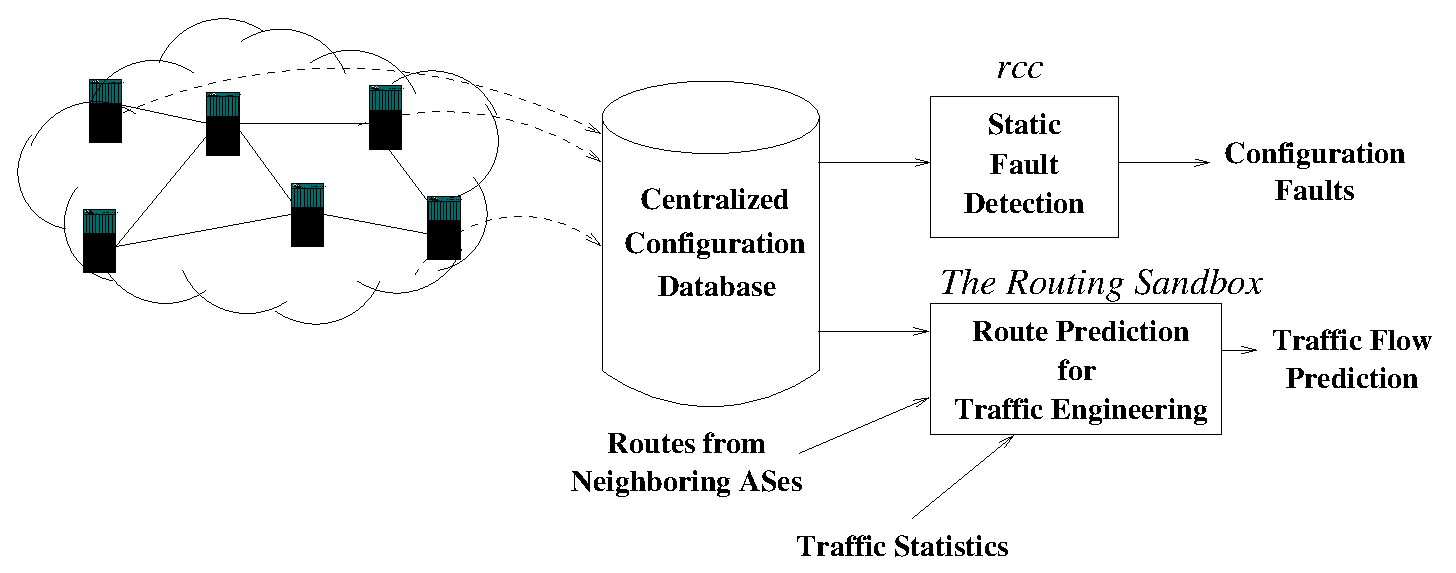
\epsfig{file=figures/process.eps, width=0.9\linewidth}
\caption[Workflow for fault detection and route prediction
  tasks.]{Workflow for fault detection and route prediction tasks 
  described in this dissertation. Both fault detection and route
  prediction tasks rely on {\em offline} analysis of the distributed 
  router configurations, which are first collected into a centralized
  database.}
\label{fig:intro:process}
\end{figure}


This dissertation presents two complementary systems that advance the
state-of-the art in fault detection and traffic engineering,
respectively.  Figure~\ref{fig:intro:workflow2} shows how these two
systems change the workflow of configuring routers.  Both of these new
systems analyze the {\em static} router configuration files.  We first
describe \rccns, a fault detection system for router configurations.  We
then describe the {\em routing sandbox}, a tool that predicts how traffic
will flow through an AS, given only a static snapshot of the router
configurations.  Together, these contributions assist a network operator
in detecting faulty routing configurations and determine the effects of
a configuration on traffic flow.

Because the techniques we present predict the behavior of the routing
protocol before it even runs, the techniques we present directly analyze
of the static configuration files.  Figure~\ref{fig:intro:process}
illustrates this process.  The configurations from the routers within an
AS are first collected from the routers and stored in a central
database.  Fault detection is performed by executing queries directly
against this repository (Chapter~\ref{chap:rcc} provides more details).
Route prediction for traffic engineering (Chapter~\ref{chap:sandbox}) is
performed in a similar fashion, but also requires additional inputs:
computing the routes that each router selects requires knowing which
routes each router learns from neighboring ASes in the first place.
Once the route that each router ultimately selects is computed, an
operator could use traffic statistics to determine the utilization on
each link in the network, but this dissertation does not address this
problem.

\subsubsection{\rccns: Proactive fault detection for Internet routing
configuration}

Chapter~\ref{chap:rcc} presents the design and implementation of \rccns,
the ``router configuration checker'', a tool that uses static 
configuration analysis to detect faults in the routing configurations
within a single AS.  We designed \rcc starting with the correctness
specification as a guide and determining the constraints on the 
aspects of configuration (described in more detail in
Section~\ref{sec:semantics}) that must hold to guarantee that the
higher level correctness properties are satisfied.  \rcc analyzes the
set of router configurations from a single AS and determines whether
they could induce violations of the correctness specification.  

{\em rcc} has been downloaded by over seventy network operators, and we
have personally used {\em rcc} to study faults in the
routing configurations of $17$ real-world ASes.
Chapter~\ref{chap:sandbox} presents algorithms and a tool that helps
network operators predict how a particular routing configuration will
affect the flow of traffic through the AS.  In conjunction with
{\em rcc}, this tool allows a network operator to answer critical
questions about routing configuration (\ie, whether the configuration
will cause catastrophic problems, and how it will affect the flow of
traffic through the AS) {\em before} the configuration is actually
deployed on a live network.

Our work on \rcc demonstrates that static configuration analysis can
detect a significant number of configuration faults that could cause the
routing protocol to violate correctness. Surprisingly, \rcc also
discovered many such faults in {\em deployed} routing configurations,
even those from large, well-known Internet service providers.  \rcc even
found configuration faults in ASes that use ``automated''
configuration techniques: of course, automated configuration systems
will have difficulty generating correct configuration if they do not
receive correct input in the first place.  Many of the
configuration faults that \rcc detects in practice suggest that
configuring a network 
of routers without introducing inconsistencies across router
configurations is surprisingly difficult.

%% Although \rcc uses only static analysis of routing configuration to
%% detect faults, some routing faults are best detected using analysis of
%% routing protocol dynamics in concert static configuration analysis may
%% also prove useful for detecting routing faults.  In
%% Chapter~\ref{chap:concl}, we speculate on scenarios where dynamic
%% analysis may prove useful.

\subsubsection{The Routing Sandbox: Proactive route prediction for
network engineering}

Chapter~\ref{chap:sandbox} describes algorithms that compute the effects
of a configuration change offline, given only a static snapshot of the
routing configurations and the available routes.  These algorithms can
then be combined with information about traffic demands to help network
operators determine how a particular routing configuration will affect
the flow of traffic through the AS.  Rather than simulating complex
protocol dynamics to determine the effects of configuration on route
selection, we model the {\em outcome} of BGP's route selection process.
{\em We exploit the properties of the correctness specification to
simplify this process:} assuming that \rcc has already verified that the
configuration satisfies route validity, path visibility, and safety
makes it possible to model AS-wide route selection without simulating
the dynamics of the routing protocols.

Route prediction becomes increasingly difficult in ASes that enable two
protocol ``features'': the Multiple Exit Discriminator (MED) attribute
and route reflection, which are described in
Sections~\ref{sec:propagation} and~\ref{sec:dissemination}, respectively.
We design algorithms for predicting BGP 
route selection for ASes that have any combination of these two features
enabled.  We also perform a running-time analysis of each of these
algorithms, which provides insight into how each of these features adds
complexity to Internet routing.

We have implemented these algorithms in a tool called the {\em routing
sandbox} that allows a network operator to {\em quickly} evaluate the
effects of incremental configuration changes.  This tool exploits
several unique aspects of the system inputs to optimize the computation
of routes for all destinations for every router in the AS.  We envision
that the routing sandbox could be used as an ``inner loop'' to other
tools that iteratively search through a large parameter space to find
optimal settings~\cite{Ye2003}.

\subsection{Conditions for Safety of the Global Routing System}



Configuration allows an operator to control both the route that each
router selects to a destination (\ie, {\em ranking}) and which routes
each router readvertises to neighboring routers (\ie, {\em filtering}).
One way to guarantee safety is to restrict some aspects of the
configuration's flexibility.  In Chapter~\ref{chap:policy}, we derive
necessary and sufficient conditions on the policies of each AS that
guarantee safety
if each AS independently follows these constraints.  Specifically, we
explore how each AS 
must restrict rankings to guarantee that the global routing system
satisfies safety, assuming that no AS wants to share its rankings with
any other AS, and no AS's rankings should be constrained by the rankings
of another AS (that is, each AS should retain {\em autonomy}).

We show that any protocol that does not restrict the business
arrangements of how ASes exchange routes with one another must impose
strong restrictions on how ASes are allowed to express preferences over
candidate routes for a destination.
%
Initially, this finding may sound rather grim, because shortest paths
routing may not provide network operators sufficient flexibility to
achieve their economic and performance goals.  On the contrary, the
results we present in this dissertation should be viewed as a first cut
towards designing routing protocols that are guaranteed to satisfy
safety, regardless of how they are configured.  Today, network operators
have no way to reason about the stability of the routing protocol, so
they are left to {\em ad hoc} methods for determining whether routing
updates correspond to unintended interactions.  A routing protocol that
conforms to the guidelines we outline in Chapter~\ref{chap:policy}
guarantees that changes in the routing protocol always reflect changes
in the underlying topology, thereby facilitating troubleshooting.
Furthermore, designing a protocol that is guaranteed to satisfy safety
on a fast timescale allows conflicts of business policy to be resolved
{\em outside} the protocol, rather than being reflected as oscillations
within the protocol itself.


\section{Lessons Learned}\label{sec:lessons}

This dissertation provides the following important lessons that can aid
the networking community as it considers proposals for evolving the
Internet routing infrastructure.

\subsection{Static configuration analysis detects many faults}

\rcc detected configuration faults in the routing configurations of all 17
ASes we analyzed and more than a thousand faults overall.  It may
seem surprising that \rcc was able to detect configuration faults in
{\em deployed} routing configurations.  In fact, this finding
demonstrates that there are many potentially catastrophic configuration
faults that do not immediately cause routing failures when they are
deployed.

The fact that static analysis can find important configuration faults
without overwhelming network operators with a vast quantity of false
positives is also somewhat remarkable.  \rcc does {\em not} operate with
a specification of the routing protocol's intended behavior.  Rather, it
operates solely on the routing configurations that {\em implement} an
operator's intent with low-level mechanisms.  Ideally, \rcc would check
the router configurations against a high-level specification of intended
behavior.  It is noteworthy that \rcc can provide a useful tool to
network operators in the absence of such a specification.

Configuration languages may ultimately evolve to make certain types of
configuration faults less likely, but static configuration analysis will
remain a crucial step in the workflow of network operations.  We believe
that the more mechanistic aspects of routing configuration will
ultimately be supplanted with high-level policy specification.  For
example, preventing routes that were learned from one neighboring
AS from being advertised to another today requires configuring
low-level, mechanistic operations on every router that exchanges routes
with either of those ASes.  Such a simple policy would better be
expressed in a specification language and ``compiled'' to the statements
that implement the mechanisms on the routers themselves.  However,
because Internet routing must always afford a network operator
flexibility in controlling the behavior of the protocol, static
configuration analysis will be invaluable for detecting faults and
evaluating routing protocol behavior, {\em
regardless of the configuration language}.  

\subsection{Distributed routing configuration leads to errors}

Our study of configuration faults in Chapter~\ref{chap:rcc}
(Section~\ref{sec:evaluation}) demonstrates
that most configuration faults result from the fact that routing
protocol configuration is {\em distributed} across the routers in the
AS.  This approach naturally causes operators to make mistakes because
it is more natural to think of the AS {\em as a whole} as implementing
some certain task (\eg, controlling traffic flow, implementing
contractual arrangements, etc.) rather than reasoning about what each
router must do to implement such a task.  A better approach may be to
allow operators to configure the AS as a monolithic entity from a
single location.

Of course, a crucial open research challenge upon which this goal
depends is what that centralized language should look like, and how the
routers themselves should implement the directives in that language.
Recent work in constraint satisfaction for network configuration
presents a possible starting point for a centralized configuration
language that satisfies high-level specification~\cite{Narain2004}.

A logically centralized routing infrastructure could act as
a catalyst for such a centralized configuration language.  For example,
a network operator could configure the AS from the RCP, which could
either (1)~compile this high-level specification into low-level router
configurations, and {\em push the configuration} to the individual
routers or (2)~select the routes on behalf of each router and {\em push
the routes} themselves to the routers.

\subsection{Safety + Autonomy $\Rightarrow$ Tight restrictions on
expressiveness} 

The (strict) conditions we derive in Chapter~\ref{chap:policy} for
guaranteeing safety suggest several possible ways for evolving the
Internet routing infrastructure.  One possibility is to relax the
autonomy requirement, by allowing groups of ASes to share certain
properties about their rankings with one another (although likely not the
rankings themselves).  Recent work has begun exploring this possibility
by recognizing that some ASes may have rankings that are more expressive
as long as others are not and designing ways to guarantee these global
properties without requiring ASes to divulge sensitive information about
rankings~\cite{Machiraju2004}.  One area for future work to determine
the information that must be shared (and with what other ASes it must be
shared) to detect and {\em resolve} safety violations, and, in
general, to study the tradeoffs between safety and the autonomy and
privacy of an ASes rankings.

Another possibility for evolving the Internet routing system is to
restrict expressiveness so that rankings must be consistent with
shortest paths routing, but allow each AS to control the weights on
edges incident to itself.  Such a routing protocol would always
satisfy safety (even assuming ASes are allowed to filter routes
arbitrarily), and any
%but the protocol may converge to a path assignment that a
%network operator does not want, hence causing the operators of each
%AS to repeatedly fiddle with rankings.  If a set of ASes have a
%legitimate policy conflict (\eg, a set of ASes all prefer routes through
%each other, thus creating a cycle of preferences), the protocol would
%then oscillate in accordance with network operators updating their
%rankings.  Such 
policy disputes could then be resolved with a negotiation protocol that
operates independently of the routing protocol, where routing updates
would only reflect actual changes in the network topology.  We explore
this possibility and others in detail in
Chapter~\ref{chap:policy} (Section~\ref{sec:policy:implications}).
 

\subsection{Protocol design should consider correctness and
predictability}\label{sec:mods} 

This dissertation focuses on improving the correctness and
predictability of the current Internet routing system, but a major
lesson from our work is that many of the tools and techniques that we
develop in the coming chapters could have been much simpler had the
protocol been designed with correctness and predictability in mind in
the first place.  

To this end, this dissertation proposes several minor modifications to
the Internet routing protocol that would have simplified the task of
achieving correct and predictable behavior.  These modifications are
minor in the sense that they can be implemented with no modifications to
routers or routing protocol specifications; on the other hand, they are
significant because they eliminate the artifacts that result from the
two most troublesome aspects of BGP: route reflection and the ``multiple
exit discriminator'' (MED) attribute.  In summary, we will see that
these two artifacts are responsible for much of the undesirable behavior
in Internet routing, ranging from persistent oscillation to network
partitions.  
%% In Chapters~\ref{chap:policy} and~\ref{chap:sandbox}, we will see that
%% much of the complexity of predicting the outcome of BGP route selection
%% is caused by route reflection, the MED attribute, and the interaction
%% between these two artifacts.  While MED serves a useful purpose in
%% allowing one AS to express preferences over exit points to its neighbor,
%% it also can create protocol oscillations, because the presence or
%% absence of some route can affect a router's relative preference between
%% two {\em different} routes.  This behavior arises because different
%% neighboring ASes may assign different MED values; as a result, a router
%% can only compare the MED values among routes from the {\em same} AS for
%% that destination, not across all routes for that destination.  In
%% Chapter~\ref{chap:sandbox} (Section~\ref{sec:sandbox:med_disc}), we
%% propose a small modification to BGP configuration that allows the MED
%% attribute to be compared across all routes to a destination (thus
%% eliminating the possibility for MED-induced oscillations) but still
%% preserves the ability for a neighboring AS to express relative
%% preferences over exit points.

One logical conclusion that can be drawn from the work in
this dissertation is that, rather than trying to {\em infer} the
protocol's behavior, the Internet routing system should provide more
direct {\em control} over route selection.
%
This insight is central to the Routing Control Platform (RCP) proposal,
which we describe briefly in Section~\ref{sec:rcp}.  RCP takes as input
the routes that an AS learns from neighboring ASes and the network
configuration, and computes routes on behalf of each router in the AS.
In some sense, RCP can be viewed as the logical extension to the routing
sandbox: RCP takes roughly the same inputs as the sandbox, but rather
than simply computing the routes that each router would select, RCP
actually controls route selection.

%% RCP
%% ensures that the route assignments for each router are based on a
%% complete view of the AS topology, and that routers are selecting paths
%% through the AS in a consistent fashion, thereby preventing forwarding
%% loops, blackholes (\ie, instances where traffic arrives at a router that
%% has no routing table entry for it), etc.  Recent work has demonstrated
%% that RCP can be used to perform route selection on behalf of all of the
%% routers in a large tier-1 ISP~\cite{caesar2004}, but many questions
%% remain.  Chapter~\ref{chap:concl} (Section~\ref{sec:rcp}) presents an
%% initial design of RCP and discusses the various benefits it could
%% provide (as well as open questions).

%\subsection{Eliminating MED while retaining its benefits} 





\section{How to Read This Dissertation}\label{sec:guide}

The problems with today's Internet routing infrastructure suggest one of
two attitudes:

\begin{enumerate}
\item Accept the Internet routing architecture ``as is'' and retrofit
  correctness and predictability by providing tools and techniques that
  make network operations less prone to faults and more predictable.
\item Adapt the routing architecture to make incorrect behavior
  less likely in the first place.
\end{enumerate}

Various parts of this dissertation cater to each of these philosophies.
The former philosophy can have more immediate impact and in fact can
provide ``bottom up'' insight regarding what aspects of the routing
architecture are most problematic.  Chapters~\ref{chap:rcc}
and~\ref{chap:sandbox} adopt this philosophy by providing tools and
algorithms that have helped network operators {\em today}.  \rcc has
been downloaded by over seventy network operators and has successfully
detected faults in the configurations of many large backbone Internet
Service Providers.  Additionally, the faults that \rcc uncovered in our
analysis of 17 real-world ASes, as well as the various aspects of BGP
that contribute complexity to the algorithms in
Chapter~\ref{chap:sandbox}, have helped us identify the aspects of the
routing architecture that beg for improvement.

Chapter~\ref{chap:policy} explores possibilities for improving routing
stability that will most likely require fundamental changes to the
Internet routing architecture because the conditions for stability would
require changing the configuration ``knobs'' that are exposed to network
operators.  The problems examined in this chapter use restrictions on
{\em static} configuration of the routing protocol to guarantee stable
dynamics.  
%% Section~\ref{sec:rcp} moves beyond simple static analysis,
%% proposing a fundamentally new mechanism for disseminating routes within
%% an AS and opening up new possibilities (as well as many unanswered
%% questions) for network management and configuration.

This dissertation caters both to the theoretician and the practitioner.
Chapter~\ref{chap:rlogic} presents a correctness specification for
Internet routing that could appeal to both parties.  Those most interested in
practical applications should focus primarily on Chapters~\ref{chap:rcc}
and~\ref{chap:sandbox}; Chapter~\ref{chap:policy} has fewer immediate
practical applications, but will be of interest to those interested in
fundamental results on routing stability and safety.  At the end of
Chapters~\ref{chap:rcc},~\ref{chap:sandbox}, and~\ref{chap:policy}, we
explore possibilities for 
evolving the Internet infrastructure to make the problems we solve
easier in the future; these sections should also have broad appeal.

%a thorough treatment (and
%hopefully lucid explanation) of Internet routing stability.
